%%%%%%%%%%%%%%%%%%%%%%%%%%%%%%%%%%%%%%%%%%%%%%%%%%%%%%%%%%%%%%%%%%%%%%%%%%%
% MENO:             ITY Projekt 3 - Tabulky a obrázky
% AUTOR:            Filip Novak
% XLOGIN:           xnovakf00
% DATUM:            22-03-2024
% POSLEDNA UPRAVA:  03-04-2024 19:58
%%%%%%%%%%%%%%%%%%%%%%%%%%%%%%%%%%%%%%%%%%%%%%%%%%%%%%%%%%%%%%%%%%%%%%%%%%%

\documentclass[a4paper, 11pt]{article}
    \usepackage[left=2cm, top=3cm, text={17cm,24cm}]{geometry}
    \usepackage[utf8]{inputenc}
    \usepackage[T1]{fontenc}
    \usepackage[czech]{babel}
    \usepackage{times}
    \usepackage{hyperref}
    \usepackage{multirow}
    \usepackage{graphics}
    \usepackage[linesnumbered,czech,ruled]{algorithm2e}
    \usepackage{pdflscape}
    \usepackage{picture}

\begin{document}

\begin{titlepage}
    \begin{center}
        \textsc{\Huge{Vysoké učení technické v~Brně\\[0.4em]}
        \huge{Fakulta informačních technologií}}\\        
        \vspace{\stretch{0.382}}
        \LARGE{Typografie a~publikování\,--\,3. projekt}\\
        \Huge{Tabulky a~obrázky}\\
        \vspace{\stretch{0.618}}
    \end{center}
    \Large{\today\hfill Filip Novák}
\end{titlepage}

\section{Úvodní strana}
Název práce umístěte do zlatého řezu a~nezapomeňte uvést dnešní datum a~vaše jméno a~příjmení.

\section{Tabulky}\label{tabulky}
Pro sázení tabulek můžeme použít buď prostředí\texttt{ tabbing }nebo prostředí\texttt{ tabular}.
\subsection{Prostředí\texttt{ tabbing }}
Při použití\texttt{ tabbing }vypadá tabulka následovně:
\begin{tabbing}
    Vodní melouny \quad\=35{,}--\qquad \=1 kus \kill
    \textbf{Ovoce} \> \textbf{Cena} \> \textbf{Množství}\\
    Jablka \> 25{,}90 \> 3\,kg\\
    Hrušky \> 27{,}40 \> 2{,}5\,kg\\
    Vodní melouny \> 35{,}-- \> 1 kus\\
\end{tabbing}

\noindent Toto prostředí se dá také použít pro sázení algoritmů, ovšem vhodnější je použít prostředí\texttt{ algorithm }nebo
\texttt{ algorithm2e }(viz sekce \ref{algo}).

\subsection{Prostředí\texttt{ tabular }}
Další možností, jak vytvořit tabulku, je použít prostředí\texttt{ tabular}. Tabulky pak budou vypadat takto\footnote{Kdyby byl problem s\texttt{ cline,} zkuste se podívat třeba sem: \href{http://www.abclinuxu.cz/tex/poradna/show/325037}{http://www.abclinuxu.cz/tex/poradna/show/325037}.}:
\\
\begin{table}[ht]
\catcode`\-=12 % for cline fix
\begin{center}
\begin{tabular}{| l | c | c |} 
    \hline
    & \multicolumn{2}{c |}{\textbf{Cena}}\\
    \cline{2-3}
    \textbf{Měna} & \textbf{nákup} & \textbf{prodej}\\
    \hline
    EUR & 25,475 & 27,045 \\
    GBP & 28,835 & 30,705 \\
    USD & 22,943 & 24,357 \\
    \hline
\end{tabular}
\caption{Tabulka kurzů k~dnešnímu dni}
\label{kurz}
\end{center}
\end{table}
\begin{table}[ht]
    \catcode`\-=12
\centering
\begin{tabular}{| c | c |}
    \hline
    $A$ & $\neg A$\\
    \hline
    \textbf{P} & N\\
    \hline
    \textbf{O} & O\\
    \hline
    \textbf{X} & X\\
    \hline
    \textbf{N} & P\\
    \hline
\end{tabular}
\begin{tabular}{| c | c | c | c | c | c |}
    \hline
    \multicolumn{2}{| c |}{\multirow{2}{*}{$A \land B$}} & \multicolumn{4}{ c |}{$B$} \\
    \cline{3-6}
    \multicolumn{2}{| c |}{} & \textbf{P} & \textbf{O} & \textbf{X} & \textbf{N} \\
    \hline
    \multirow{4}{*}{$A$}
    & \textbf{P} & P & O & X & N \\
    \cline{2-6}
    & \textbf{O} & O & O & N & N \\
    \cline{2-6}
    & \textbf{X} & X & N & X & N \\
    \cline{2-6}
    & \textbf{N} & N & N & N & N \\
    \hline
\end{tabular}
\begin{tabular}{| c | c | c | c | c | c |}
    \hline
    \multicolumn{2}{| c |}{\multirow{2}{*}{$A \lor B$}} & \multicolumn{4}{ c |}{$B$} \\
    \cline{3-6}
    \multicolumn{2}{| c |}{} & \textbf{P} & \textbf{O} & \textbf{X} & \textbf{N} \\
    \hline
    \multirow{4}{*}{$A$}
    & \textbf{P} & P & P & P & P \\
    \cline{2-6}
    & \textbf{O} & P & O & P & O \\
    \cline{2-6}
    & \textbf{X} & P & P & X & X \\
    \cline{2-6}
    & \textbf{N} & P & O & X & N \\
    \hline
\end{tabular}
\begin{tabular}{| c | c | c | c | c | c |}
    \hline
    \multicolumn{2}{| c |}{\multirow{2}{*}{$A \rightarrow B$}} & \multicolumn{4}{ c |}{$B$} \\
    \cline{3-6}
    \multicolumn{2}{| c |}{} & \textbf{P} & \textbf{O} & \textbf{X} & \textbf{N} \\
    \hline
    \multirow{4}{*}{$A$}
    & \textbf{P} & P & O & X & N \\
    \cline{2-6}
    & \textbf{O} & P & O & P & O \\
    \cline{2-6}
    & \textbf{X} & P & P & X & X \\
    \cline{2-6}
    & \textbf{N} & P & P & P & P \\
    \hline
\end{tabular}
\caption{Protože Kleeneho trojhodnotová logika už je \uv{zastaralá}, uvádíme si zde příklad čtyřhodnotové logiky}\label{log}
\end{table}

\section{Algoritmy}\label{algo}
Pokud budeme chtít vysázet algoritmus, můžeme použít prostředí\texttt{ algorithm\footnote{Pro nápovědu, jak zacházet s~prostředím\texttt{ algorithm,} můžeme zkusit tuhle stránku:\\
\href{http://ftp.cstug.cz/pub/tex/CTAN/macros/latex/contrib/algorithms/algorithms.pdf}{http://ftp.cstug.cz/pub/tex/CTAN/macros/latex/contrib/algorithms/algorithms.pdf}.} }nebo\texttt{ algorithm2e\footnote{Pro\texttt{ algorithm2e }zase tuhle: \href{http://ftp.cstug.cz/pub/tex/CTAN/macros/latex/contrib/algorithm2e/doc/algorithm2e.pdf}{http://ftp.cstug.cz/pub/tex/CTAN/macros/latex/contrib/algorithm2e/doc/algorithm2e.pdf}.}}.
Příklad použití prostředí\texttt{ algorithm2e }viz Algoritmus \ref{fastslam}.\\
\IncMargin{1.7em}
\begin{algorithm}[ht]
    \SetAlgoNoLine
    \SetNlSty{}{}{:}
    \SetAlgoNlRelativeSize{-1}
    \DontPrintSemicolon
    \SetKwFor{For}{for}{do}{end\,for}
    \Indm\Indmm
    \KwIn{$(X_{t-1}, u_t, z_t)$}
    \KwOut{$X_t$}
    \BlankLine
    \Indp\Indpp
    $\overline{X_t} = X_t = 0$\;
    \For{$k = 1$ \emph{to} $M$}
    {
        \Indpp
        $x_t^{[k]} =  \emph{sample\_motion\_model}(u_t, x_{t-1}^{[k]})$\;
        $\omega_t^{[k]} =  \emph{measurement\_model}(z_t, x_t^{[k]},m_{t-1})$\;
        $m_t^{[k]} = updated\_occupancy\_grid(z_t, x_t^{[k]},m_{t-1}^k)$\;
        $\overline{X_t} = \overline{X_t} + \langle x_x^{[m]}, \omega_t^{[m]} \rangle$\;
        \Indmm
    }
    \For{$k = 1$ \emph{to} $M$}
    {
        \Indpp
        draw $i$ with propability $\approx \omega_t^{[i]}$\;
        add $\langle x_x^{[k]}, m_t^{[k]} \rangle$ to $X_t$\;
        \Indmm
    }
    \KwRet{$X_t$}
    \caption{\textsc{FastSLAM\label{fastslam}}}
\end{algorithm}
\vspace{-0.8em} % Pre rozdielny výzor underscore v tabuľke (aj keď podľa môjho názoru sú použité korektné inštrukcie)
                % sa zvyšok dokumentu posunul o značnú časť. Použitie zápornej medzery mi prišlo v tomto prípade ako
                % najjednoduhšie riešenie.
\section{Obrázky}\label{obrazky}
Do našich článků můžeme samozřejmě vkládat obrázky. Pokud je obrázkem fotografie, můžeme klidně použít
bitmapový soubor. Pokud by to ale mělo být nějaké schéma nebo něco podobného, je dobrým zvykem takovýto
obrázek vytvořit vektorově.
\begin{figure}[h]
\begin{center}
    \scalebox{0.4}{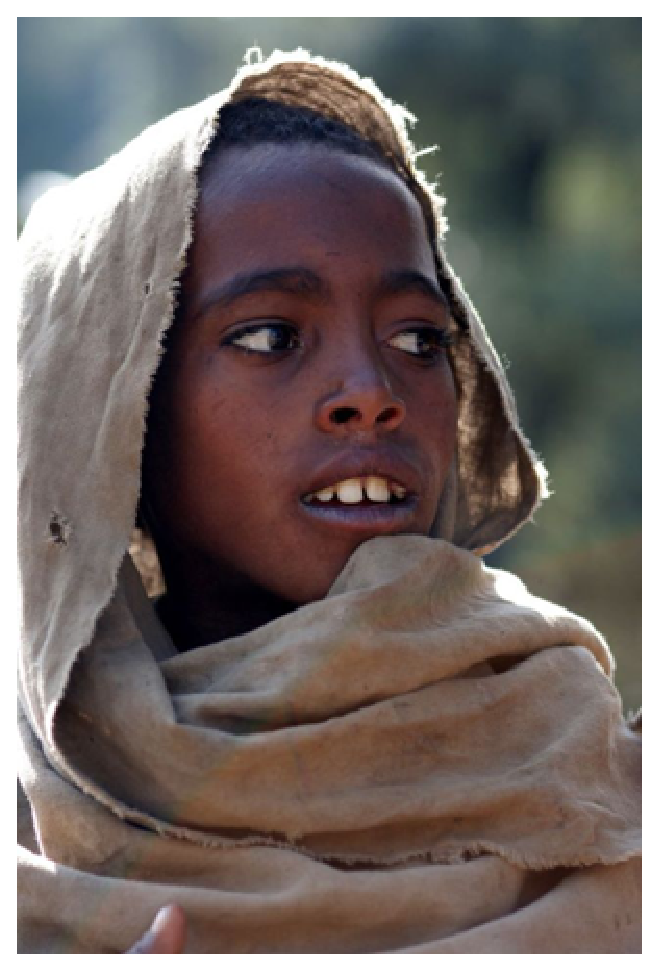
\includegraphics{etiopan.eps} \reflectbox{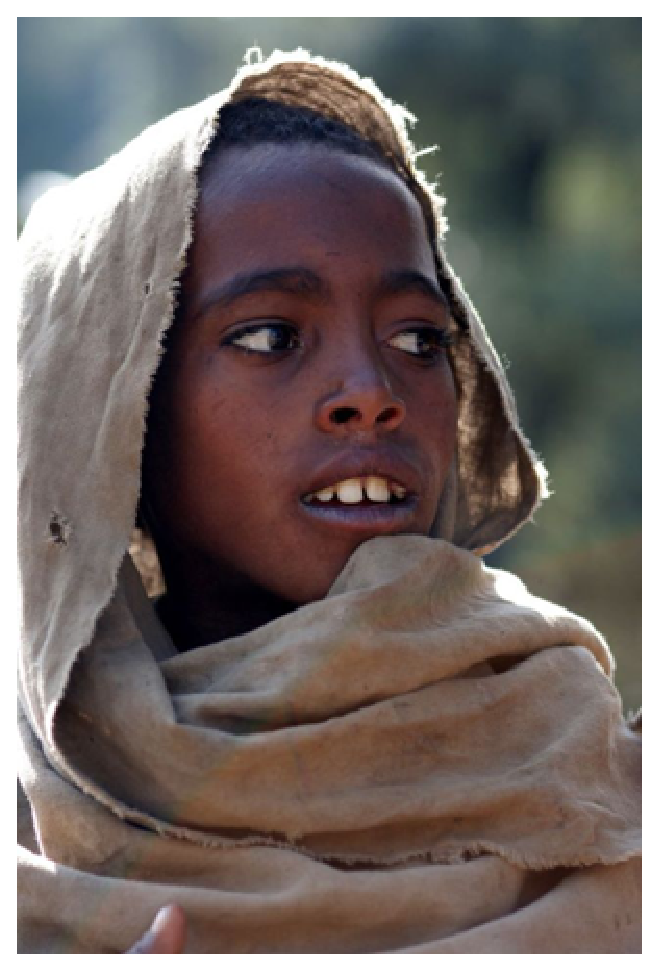
\includegraphics{etiopan.eps}}}
    \caption{Malý Etiópanek a~jeho bratříček}
    \label{etiopan}
\end{center}
\end{figure}
\pagebreak
\\
\indent Rozdíl mezi vektorovým $\dots$
\begin{figure}[h]
\begin{center}
    \scalebox{0.4}{
\includegraphics{oniisan.eps}}
    \caption{Vektorový obrázek}
    \label{oniivec}
\end{center}
\end{figure}

\noindent $\dots$ a~bitmapovým obrázkem
\begin{figure}[h]
\begin{center}
    \scalebox{0.6}{
\includegraphics{oniisan2.eps}}
    \caption{Bitmapový obrázek}
    \label{oniibit}
\end{center}
\end{figure}

\noindent se projeví například při zvětšení.

Odkazy (nejen ty) na obrázky \ref{etiopan}, \ref{oniivec} a~\ref{oniibit}, na tabulky \ref{kurz} a~\ref{log} a~také na algoritmus 1 jsou udělány pomocí křížových odkazů. Pak je ovšem potřeba zdrojový soubor přeložit dvakrát.

Vektorové obrázky lze vytvořit i~přímo v~\LaTeX u, například pomocí prostředí\texttt{ picture.}

\begin{landscape}

\begin{figure}[ht]
\begin{center}
    \setlength{\unitlength}{0.5cm}
\begin{picture}(35,25)
    \put(0,0){\framebox(35,25){}}

    % hlavne steny
    \linethickness{0.5mm}
    \put(5,4){\line(1,0){27}}
    \put(5,4){\line(0,1){9}}
    \put(25,10){\line(0,1){3}}
    \linethickness{0.1mm}

    % strecha
    \put(4,12){\line(1,1){11}}
    \put(4,13){\line(1,1){11}}
    \put(4,12){\line(0,1){1}}

    \put(15,23){\line(1,-1){11}}
    \put(15,24){\line(1,-1){11}}
    \put(26,12){\line(0,1){1}}

    % okno lave obrys
    \put(7,12){\line(0,1){2}}
    \put(7,12){\line(1,0){5}}
    \put(12,12){\line(0,1){3}}
    \put(7,14){\line(2,1){2}}
    \put(9,15){\line(1,0){3}}

    % okno lave predel
    \put(9,12){\line(0,1){3}}
    \put(10,12){\line(0,1){3}}

    % okno prave obrys
    \put(18,12){\line(1,0){5}}
    \put(18,12){\line(0,1){3}}
    \put(18,15){\line(1,0){3}}
    \put(21,15){\line(2,-1){2}}
    \put(23,12){\line(0,1){2}}

    % okno prave predel
    \put(20,12){\line(0,1){3}}
    \put(21,12){\line(0,1){3}}

    % okno lave dolne
    \linethickness{0.3mm}
    \put(7,7){\framebox(3,2){}}

    % okno prave dolne
    \put(18,7){\framebox(4,2){}}

    % dvere obrys
    \put(13,4){\framebox(3,5){}}

    % klucka
    \put(15.3,6.2){\circle*{0.3}}

    % dvere predel
    \linethickness{0.1mm}
    \multiput(13,4)(0.1,0){10}{\line(0,1){5}}

    % fasada hlavne
    \linethickness{0.3mm}
    \put(11,4){\framebox(21,6){}}

    % fasada dvere
    \put(26,4){\framebox(5,5){}}
    \linethickness{0.1mm}
    \multiput(28,9)(0.1,0){10}{\line(0,-1){5}}

    % komin
    \put(22,17){\line(0,1){4}}
    \put(21,18){\line(0,1){3}}

    \put(20.5,21){\framebox(2,0.5){}}

    % schody
    \put(12.5,3.5){\framebox(4,0.5){}}
    \put(12,3){\framebox(5,0.5){}}

    % slnko
    \linethickness{0.1mm}
    \put(30,21){\circle{2}}

    % zem
    \linethickness{0.4mm}
    \put(1,4){\line(1,0){32}}
\end{picture}
\caption{Vektorový obrázek moderního bydlení vhodného pro 21. století}
\end{center}
\end{figure}
\end{landscape}
\end{document}